%%%%%%%%%%%%%%%%%%%%%%%%%%%%%%%%%%%%%%%%%%%%%%%%%%%%%%%%%%%%%%%%%
% Qualificacao de Doutorado / Dept Fisica, CFM, UFSC            %
% Eduardo@UFSC - 2015                                           %
%%%%%%%%%%%%%%%%%%%%%%%%%%%%%%%%%%%%%%%%%%%%%%%%%%%%%%%%%%%%%%%%%

%:::::::::::::::::::::::::::::::::::::::::::::::::::::::::::::::%
%                                                               %
%                          Capítulo 3                           %
%                                                               %
%:::::::::::::::::::::::::::::::::::::::::::::::::::::::::::::::%

%***************************************************************%
%                                                               %
%                           Amostra                             %
%                                                               %
%***************************************************************%

\chapter{Amostra de galáxias}
\label{sec:amostra}

\section{Artigo - CALIFA, the Calar Alto Legacy Field Area survey III. Second public data
release.}

Esse artigo (Apêndice \ref{apendice:GBetal2015a}) descreve uma amostra de 200 galáxias que tiveram
seus dados liberados no segundo lançamento público de dados ({\em data-release} - DR2) do \PCAL.
Enveredando por todos as configurações de observação, procedimentos de redução dos dados, avaliação
de erros e controle de qualidade. 

Nesse artigo nosso grupo de populações estelares me encarregou de escrever os programas de análise e
gerar as imagens que usamos para avaliar a qualidade da síntese de populações estelares com o
\starlight em 170670 espectros para distintas posições em cada galáxia, além de comparar com os
resultados para a amostra do primeiro {\em data-release} (DR1). Durante a análise dos resíduos vimos
que os mesmos reduziram sensivelmente desde a última versão, além de nos ajudar a melhorar a máscara
de remoção de linhas telúricas dos espectros. Também verificamos que os erros relacionados aos
espectros observados possuem uma distribuição muito próxima a uma gaussiana, ou seja, resíduos
resultam praticamente ruído.

\section{Definição da amostra deste trabalho}
\label{sec:amostra:definicao}

Neste trabalho estamos interessados em estudar a formação estelar recente em discos de galáxias.
Nossa amostra começa contendo todas as 226176 regiões (zonas) das 305 galáxias espirais do \CAL.
Cada uma dessas zonas dessa é composta por um ou mais pixels, com um espectro resultante da soma dos
espectros destes, para que tenhamos relação sinal-ruído maior ou igual a 20 na janela de
normalização do espectro resultante. Esse procedimento, conhecido como {\em Voronoi binning}, está
detalhado, juntamente com o procedimento de derivação das propriedades estelares através do código
\starlight para cada uma das regiões destas galáxias, em \citet{CidFernandes.etal.2013a}.

\subsection{Mascarando elementos e removendo {\em outliers}}
\label{sec:amostra:mask}

Para que possamos focar nossos estudos às regiões de formação estelar, aplicamos uma máscara nos
dados selecionando as regiões que possuam:
\begin{itemize}
  \item medidas do fluxo integrado das linhas de \Hbeta, \oIII, \Halpha e \nII com relação
sinal-ruído maior do que 3;
  \item medidas para as seis propriedades comparadas neste capítulo ($\tauVS$, $\tauVN$,
$\SigmaSFR$, $\SigmaSFRN$, $\meanM{\log Z_\star}$ e $\log(O/H)$);
  \item fração de população estelar jovem ($t_\star < t_{SF}$) maior que 0.05 (5\%) ($x_Y >0.05$);
  \item $\tauV$ e $\tauVN$ maiores que 0.05;
  \item mais do que cinco zonas contribuindo para o cálculo dos perfis radiais (ver
  \ref{sec:synvsneb:amostra:rad});
  \item distância maior que 70\% do raio que contém metade da luz ({\em half-light radius} - HLR).
\end{itemize}
\noindent O que aqui chamamos de população jovem discutiremos um pouco mais adiante, na Sec.
\ref{sec:synvsneb:SFR}. última imposição é feita para que não haja contaminação por zonas
do bojo da galáxia (partes centrais onde as linhas são produzidas por diferentes fenômenos físicos,
relacionados a um núcleo ativo). Esse valor (0.7 HLR) foi definido por nossos colaboradores
analisando as curvas de brilho das galáxias e representa um valor máximo para localização de zonas
centrais. Na figura \ref{fig:histosample} podemos ver os efeitos da máscara que forma nossa
amostra. Em azul temos as 226176 regiões em 305 galáxias e, em vermelho, as 16525 zonas de 184
galáxias (19 Sa, 38 Sb, 59 Sbc, 55 Sc e 13 Sd). É notável que nossa seleção busca zonas mais compactas e
mais jovens (maior fração de populações jovens diminuindo a idade média). 
\begin{figure}
	\centering
	\resizebox{0.99\textwidth}{!}{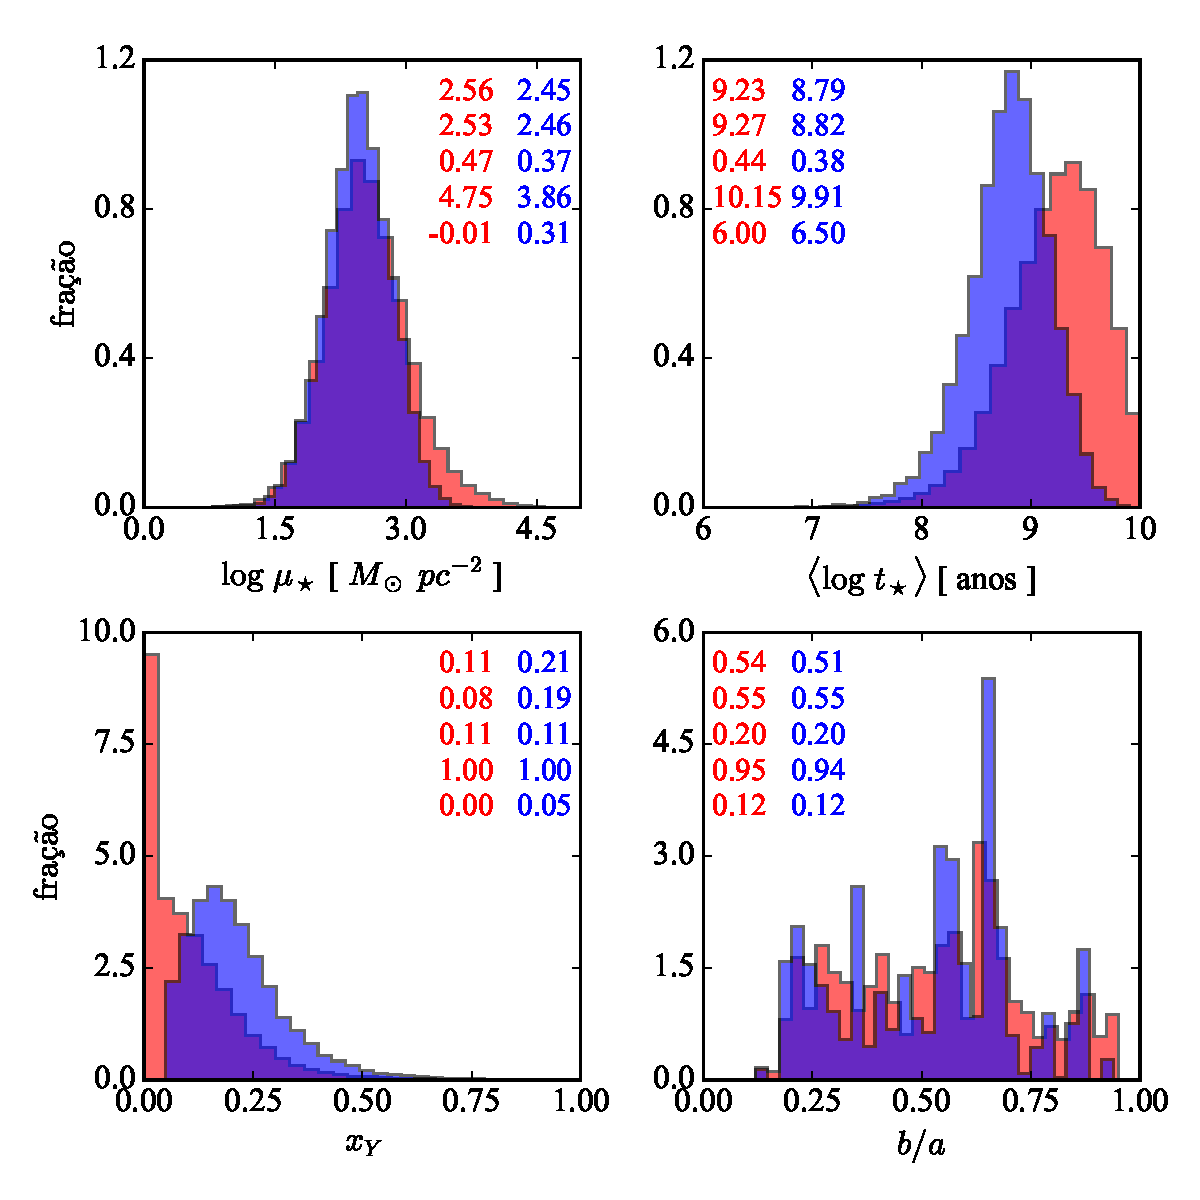
\includegraphics{figuras/histosample.pdf}}
	\caption[Histogramas: densidade superficial de massa, idade média, fração de populações jovens e
	relação axial.] 
	{Histogramas da densidade superficial de massa, idade média, fração de populações jovens e relação
axial. Em azul temos a distribuição de valores de 226176 regiões em 305 galáxias e, em vermelho, a
de 16525 zonas de 184 galáxias resultantes da seleção. Em cada gráfico temos os valores da média,
mediana, desvio padrão, máximo e mínimo de cada distribuição.}
	\label{fig:histosample}
\end{figure}

\subsection{Classificação Morfológica}
\label{sec:amostra:morf}

Com tipos morfológicos variando entre Sa e Sd, massas estelares entre $10^9$ e $10^{11.5}\ M_\odot$
e populações estelares com idades médias entre $10^8$ e $10^{10}$ anos, podemos ver na Fig.
\ref{fig:amostraMorf} que as galáxias se ordenam de forma interessante quando agrupadas por tipo
morfológico, anticorrelacionando com a idade média estelar e a massa estelar ($M_\star$ e
$t_\star$) e correlacionando com a fração de luz proveniente das população jovens ($x_Y \equiv x_Y(t_\star <
t_{SF})$). Cada galáxia contribui com um ponto em cada painel deste gráfico, ou seja, são
propriedades integradas. Os intervalos entre primeiro e terceiro quartil quase não se sobrepõem no
quando analisamos as classes morfológicas por idade média. 

Esse resultado parece ser muito interessante visto que a classificação morfológica foi feita por
colaboradores do CALIFA totalmente através de inspeção visual das imagens na banda-r do \SDSS das
mesmas galáxias. Vemos também que as galáxias tipo Sd possuem as populações estelares mais jovens e
menos massivas na média. Por ser um fenômeno apenas de posição do referencial de observação não
deveríamos ver preferência por valor de relação axial ($b/a$) quando dividimos em classes
morfológicas, o que realmente acontece.

\begin{figure}
	\centering
	%\resizebox{0.99\textwidth}{!}{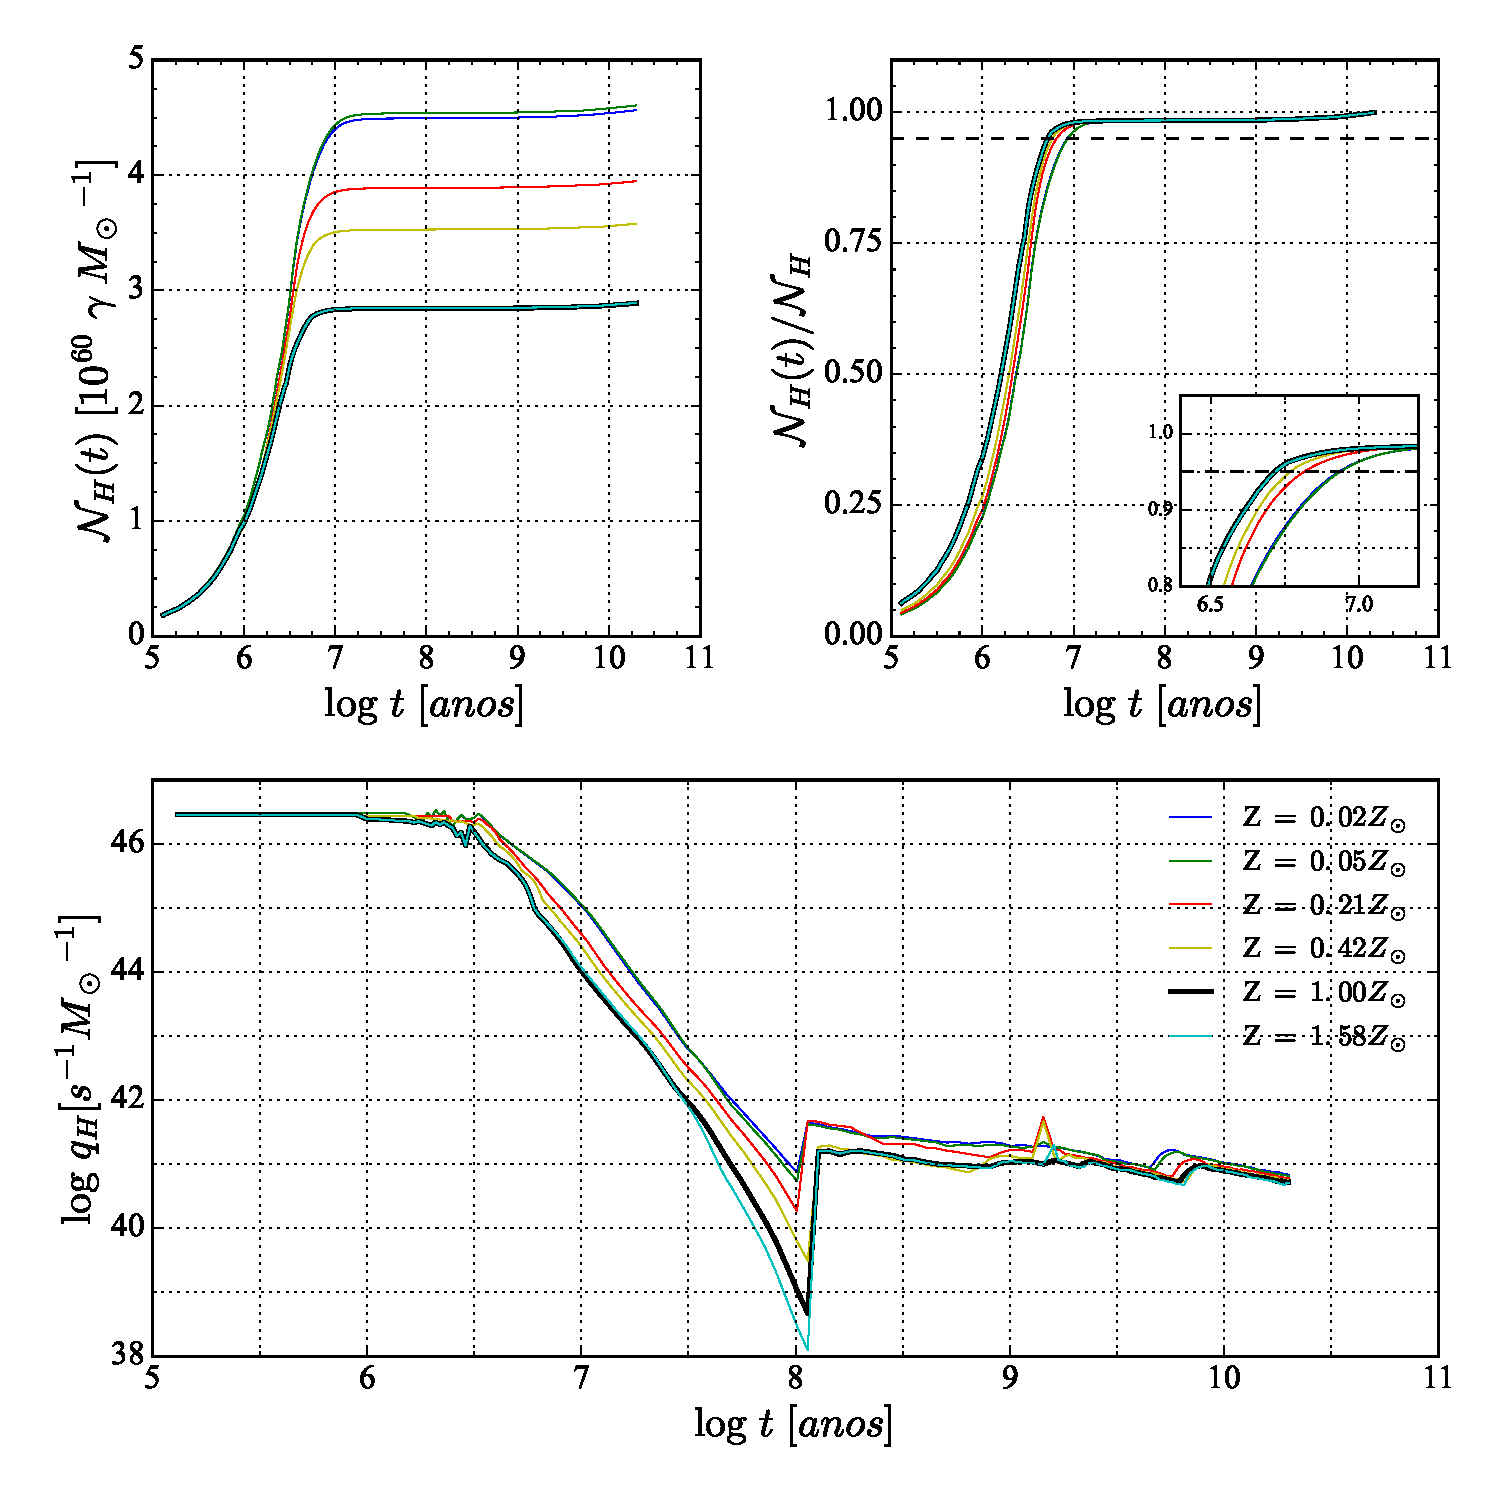
\includegraphics{Nh_logt_metBase_Padova2000_salp.pdf}}
	\resizebox{0.99\textwidth}{!}{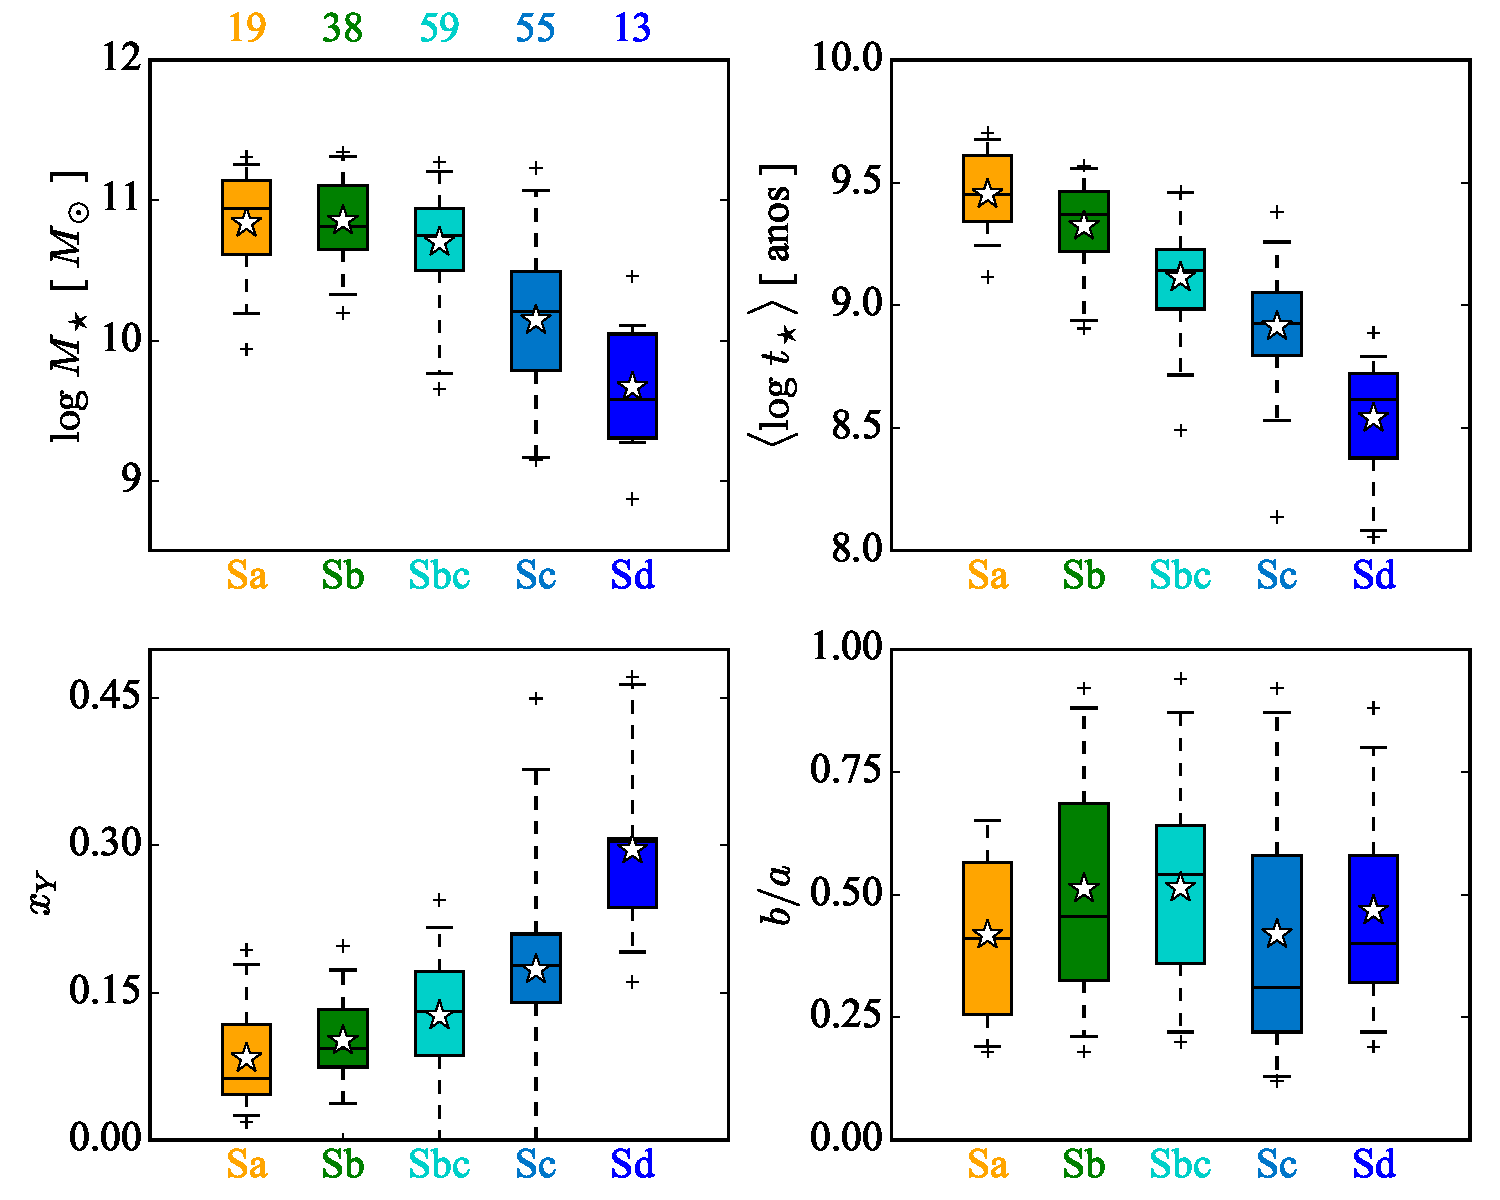
\includegraphics{figuras/sample_realsample_maskradius_integrated.pdf}}
	\caption[Classificação por morfologia.]
	{\emph{Em sentido horário a partir do painel superior esquerdo}: gráfico da massa estelar, idade
	estelar média, fração de luz proveniente das população jovens ($x_Y \equiv x_Y(t_\star < t_{SF})$) e
	inclinação, divididos em classes morfológicas para 305 galáxias espirais da amostra total do
	CALIFA. No primeiro painel, temos o número de galáxias dentro de cada classe morfológica. Cada
	caixa tem altura definida pelo primeiro e terceiro quartil da distribuição dentro de um tipo
	morfológico. Uma faixa preta marca a mediana e uma estrela a média. Em cada caixa, a linha
	pontilhada vertical se estende mostrando o intervalo de $3\sigma$. Valores que ficam fora do
	intervalo de $3\sigma$ são marcados por uma cruz vermelha.}
	\label{fig:amostraMorf}
\end{figure}

Estamos em fase de finalização de um artigo em que comparamos a relação entre a taxa de formação
estelar e a massa para diferentes classes morfológicas. Esse artigo já foi submetido e deve sair
logo agora no início de 2016.

\section{Perfis radiais}
\label{sec:amostra:rad}

Uma maneira interessante de analisar galáxias é produzir perfis radiais para as propriedades
físicas. Esse tipo de média azimutal (tanto em classes definidas por anéis circulares quanto em
anéis elípticos) diminui o espalhamento dos pontos. Para a análise individual de cada galáxia também
permite estudo da evolução das propriedades ao longo do raio. Quando colocamos todas as galáxias na
mesma análise, a vantagem dos {\em bins} radiais vem do balanceamento da influência de cada galáxia
quando analisamos todas juntas. Para que seja possível este ``empilhamento'' de galáxias, estas
médias radiais são feitas definindo-se um raio efetivo para cada galáxia. No nosso caso utilizamos
como raio efetivo aquele que comporta metade da luz da galáxia ({\em half-light radius} - HLR) e
definimos 30 anéis com espessura de 0.1 HLR (ou seja, indo até 3HLR) partindo do pixel central de
cada galáxia.

No artigo de \citet{GonzalezDelgado.etal.2014a} os autores discutem as estruturas radiais de algumas
propriedades estelares, aplicando este tipo de estudo para 107 galáxias contidas no CALIFA {\em
Survey}. Nele são derivados os raios de metade da luz (HLR) e de metade da massa ({\em half-mass
radius} - HMR) e deste resultado concluem que as galáxias são em geral 15\% mais compactas em massa
do que em luz. Também mostram que algumas propriedades, como idade estelar média, extinção por
poeira e densidade superficial de massa estelar são bem representados pelo seus valores medidas a 1
HLR.

Escolhemos utilizar perfis radiais em anéis elípticos neste trabalho, calculando a média entre todas
as zonas não mascaradas dentro de cana anel. Como um exemplo, podemos observar na Fig.
\ref{fig:K0140xYRadProf} três exemplos de mapas e perfis radiais ($x_Y$, $\tauVS$ e $\tauVN$) da
galáxia NGC1667 (objeto CALIFA 140). Em destaque (azul) temos o valor integrado para a galáxia.
Dentro de nosso trabalho utilizamos as medidas em zonas, em perfis radiais e quando necessário,
integradas (resolvendo para o disco ou para a galáxia completa), nos possibilitando portanto
verificar diferenças nestes tipos de abordagens.

\begin{figure}
	\centering
	%\resizebox{0.99\textwidth}{!}{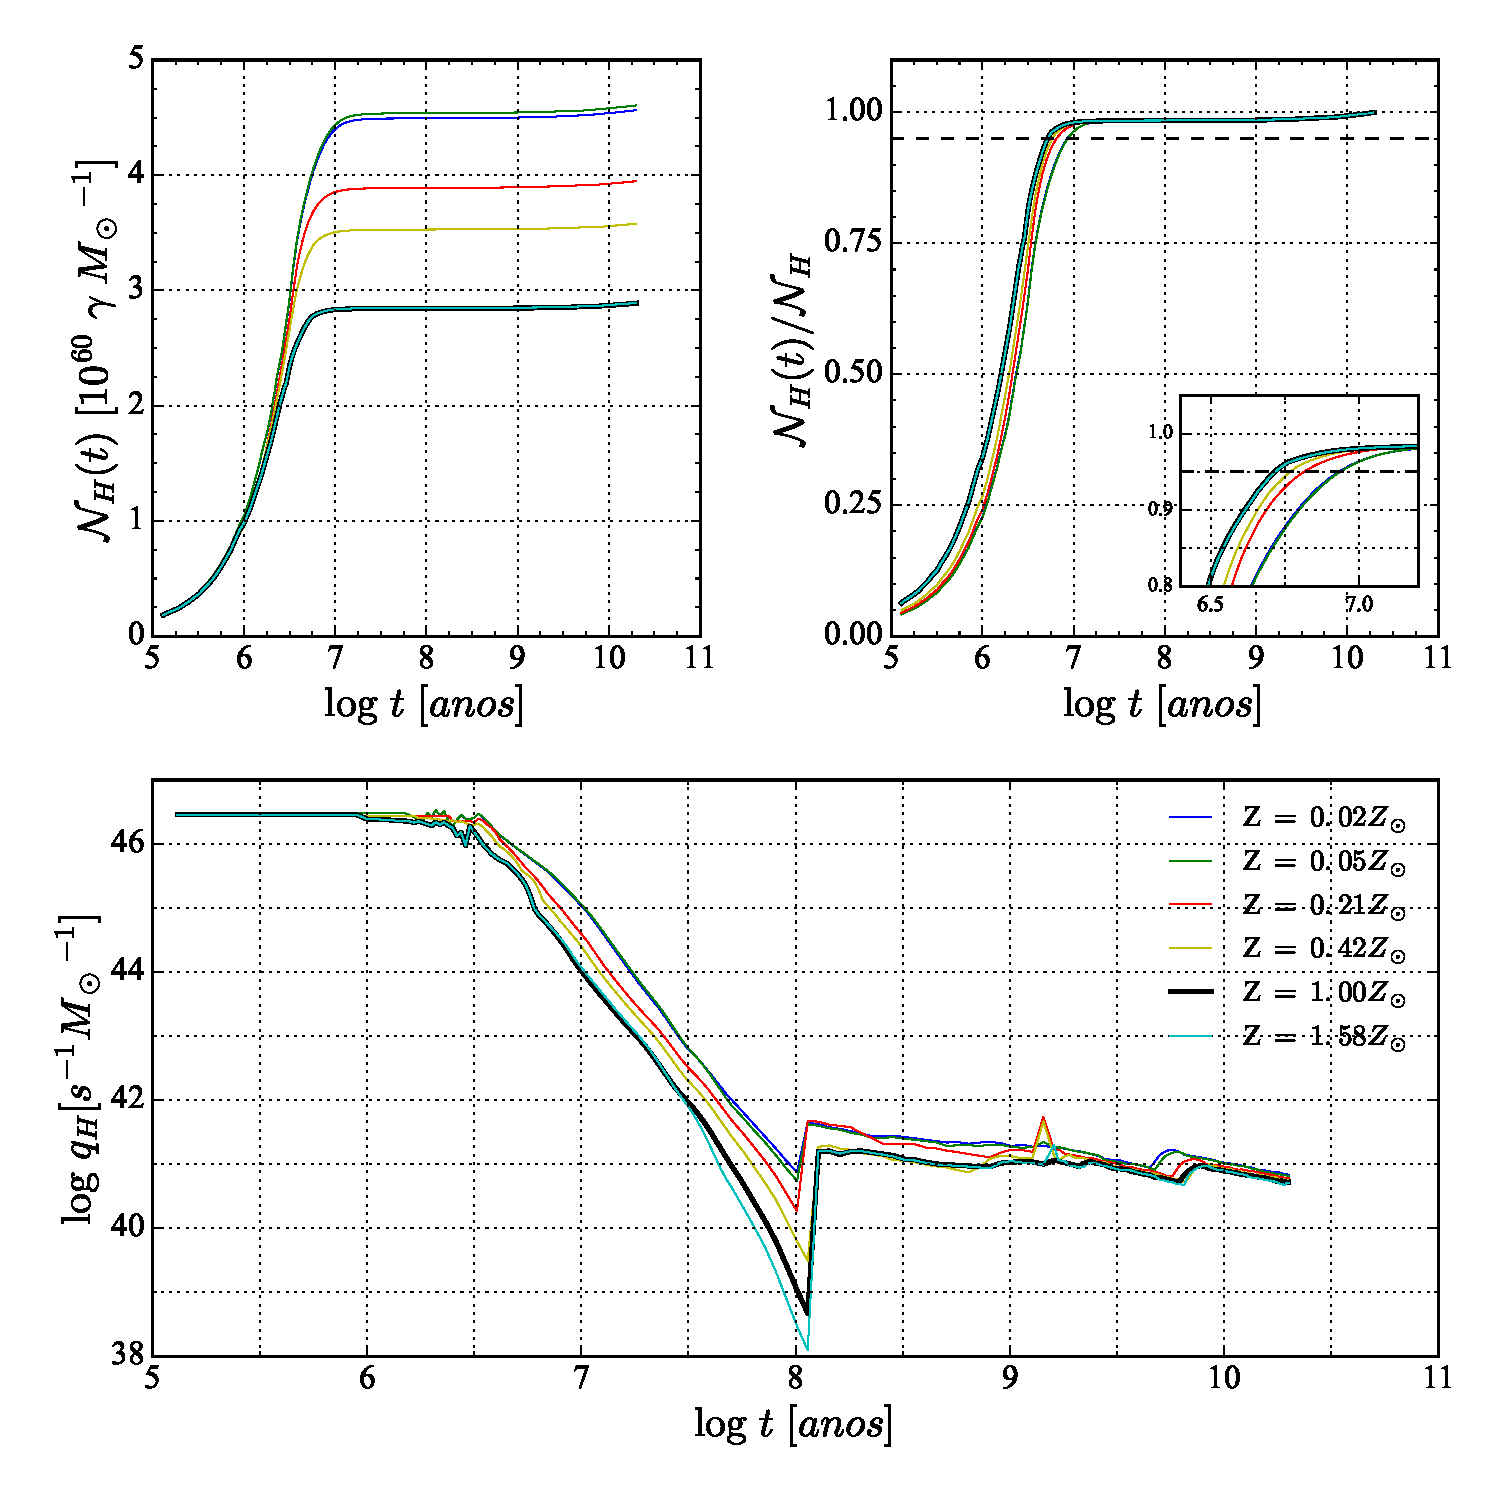
\includegraphics{Nh_logt_metBase_Padova2000_salp.pdf}}
	\resizebox{0.99\textwidth}{!}{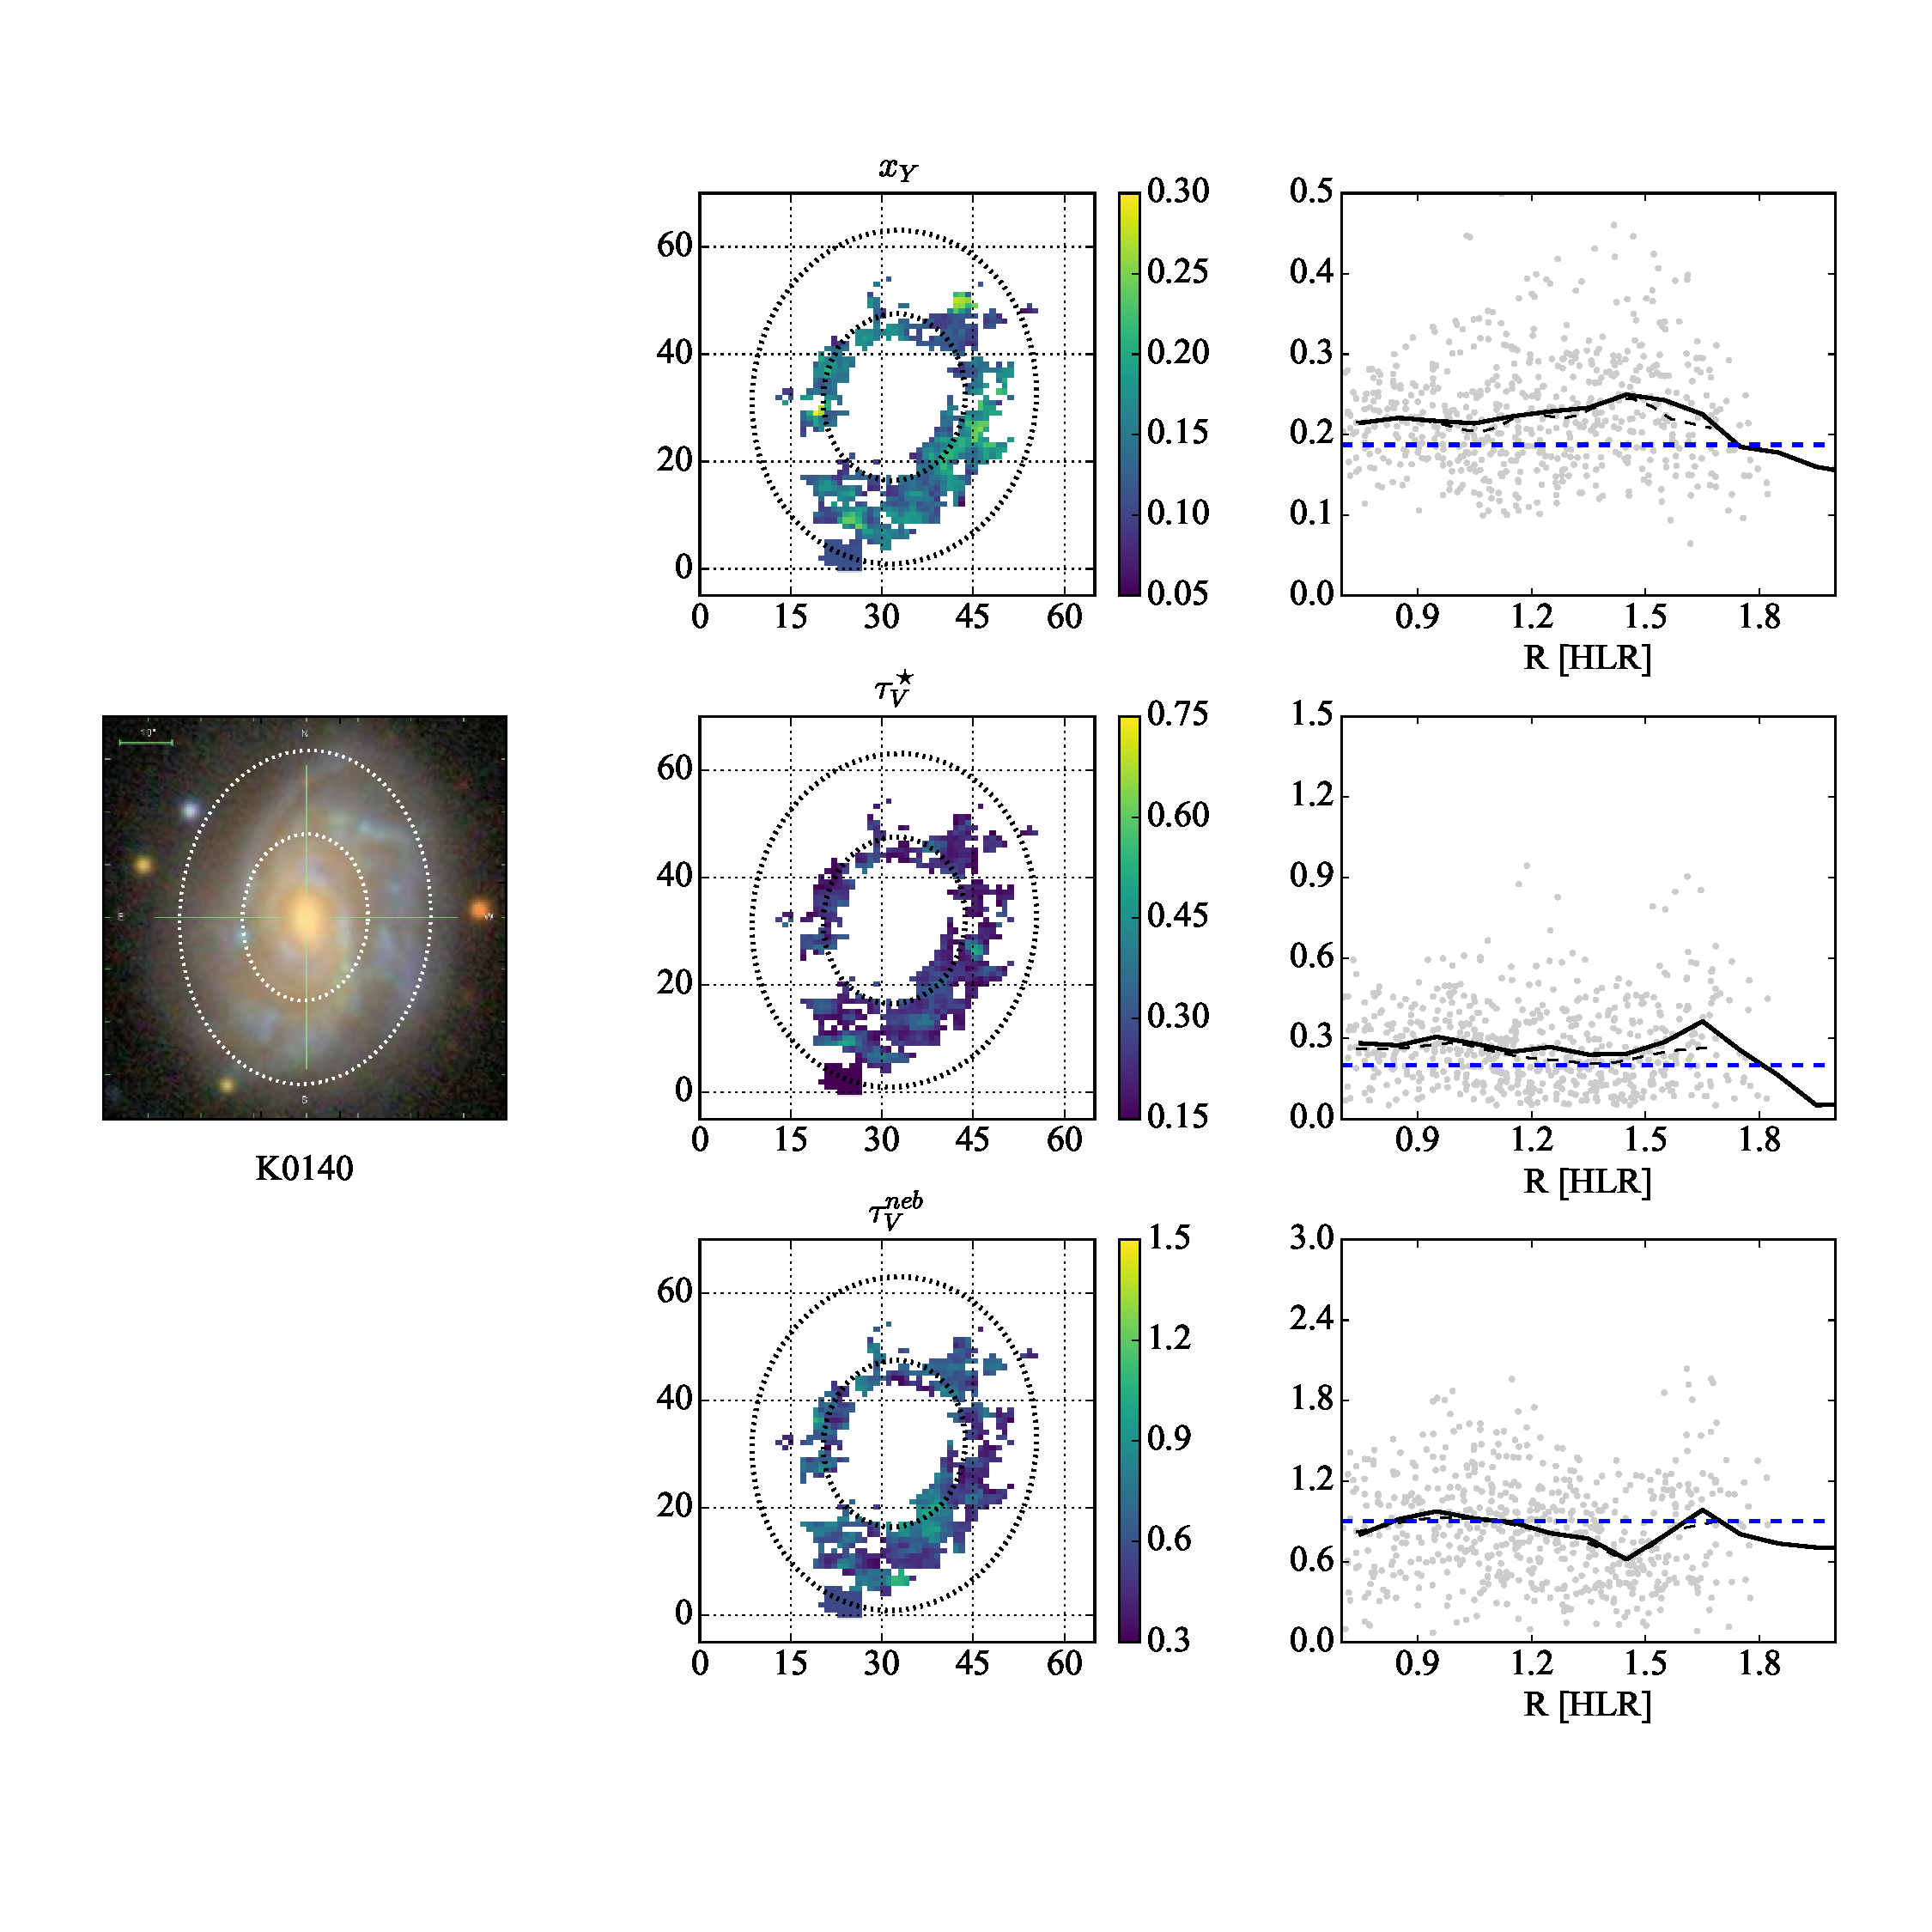
\includegraphics{figuras/K0140_xY_radialProfile_realsample.pdf}}
	\caption[Imagem e exemplos de mapas e perfis radiais.]
	{Imagem do \SDSS da galáxia NGC1667 (CALIFA 140). Em cada fileira aparece o mapa e o perfil radial
da fração de luz proveniente das populações jovens ($x_Y$ - \emph{primeira fileira}), do
coeficiente de extinção resultante da síntese de populações estelares ($\tauVS$ - \emph{segunda
fileira}) e do coeficiente de extinção por decremento de Balmer ($\tauVN$ - \emph{terceira
fileira}). Nos mapas duas elipses concêntricas marcam 1 e 2 HLR. Em cada gráfico do perfil radial
aparece no fundo em cinza os valores para as zonas, em linha tracejada preta a mediana da
distribuição ao longo do raio e em azul tracejado o valor integrado para a galáxia, além do perfil
radial (linha preta contínua).}
	\label{fig:K0140xYRadProf}
\end{figure}
 
% Figuras:
% - histograma tipos - histograma massa - influências dos cortes em tauV, raio e x_Y - Anexo: Lista
% de galáxias com massa, redshift, idade, etc ...
%% End of this chapter
